%=========================================================================
% Start of 
%=========================================================================
\preClass{Introduction to Inverse Trigonometric Functions}

\begin{problem}
\item Determine all values of $\theta$ that satisfy 
  \begin{eqnarray*}
    \sin(\theta) & = & \frac{\sqrt{2}}{2}.
  \end{eqnarray*}

  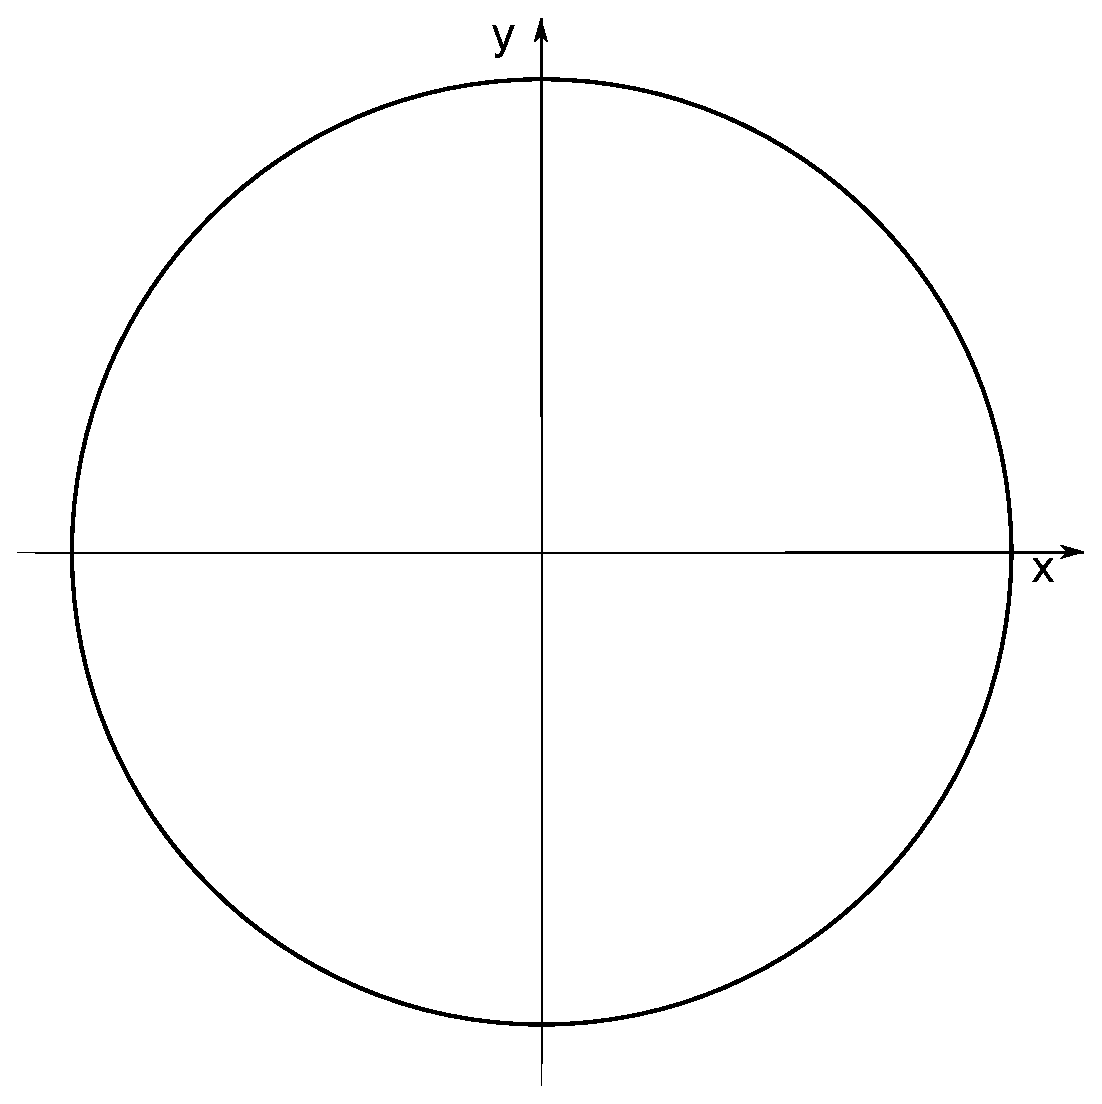
\includegraphics[width=6cm]{trig/img/blankCircle}

  Use the plot of the unit circle above, and sketch the angles that
  satisfy the equation above. Use the plot to determine the values of
  the angles in radians.

  \vfill

\end{problem}


\actTitle{Introduction to Inverse Trigonometric Functions}
\begin{problem}
\item Determine all values of $\theta$ that satisfy 
  \begin{eqnarray*}
    \cos(\theta) & = & -\frac{\sqrt{2}}{2}.
  \end{eqnarray*}

  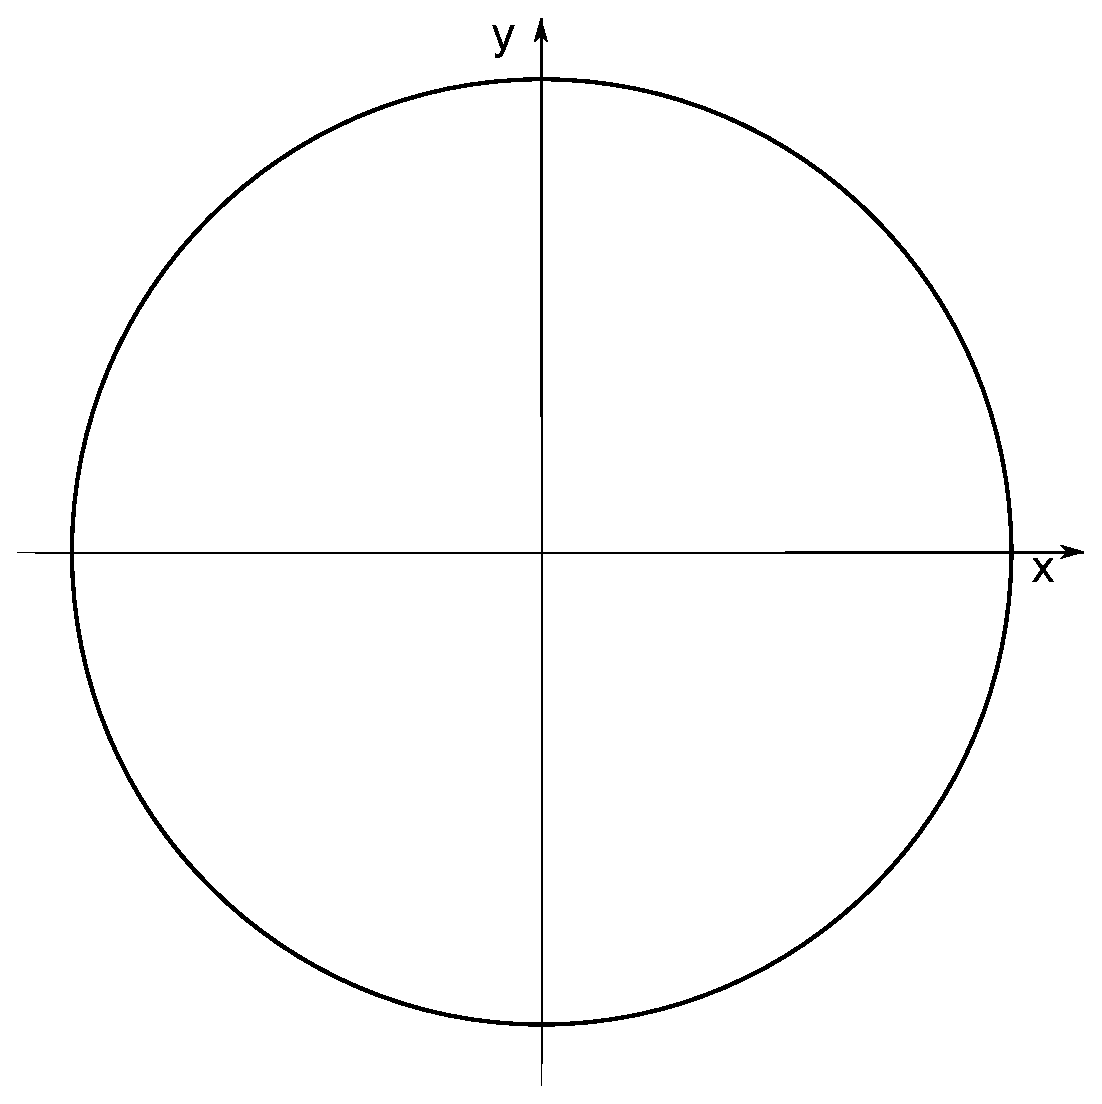
\includegraphics[width=6cm]{trig/img/blankCircle}

  Use the plot of the unit circle above, and sketch the angles that
  satisfy the equation above. Use the plot to determine the values of
  the angles in radians.

  \vfill

  \clearpage

\item Determine all values of $x$ that satisfy 
  \begin{eqnarray*}
    \cos(2x+1) & = & -\frac{\sqrt{2}}{2}.
  \end{eqnarray*}

  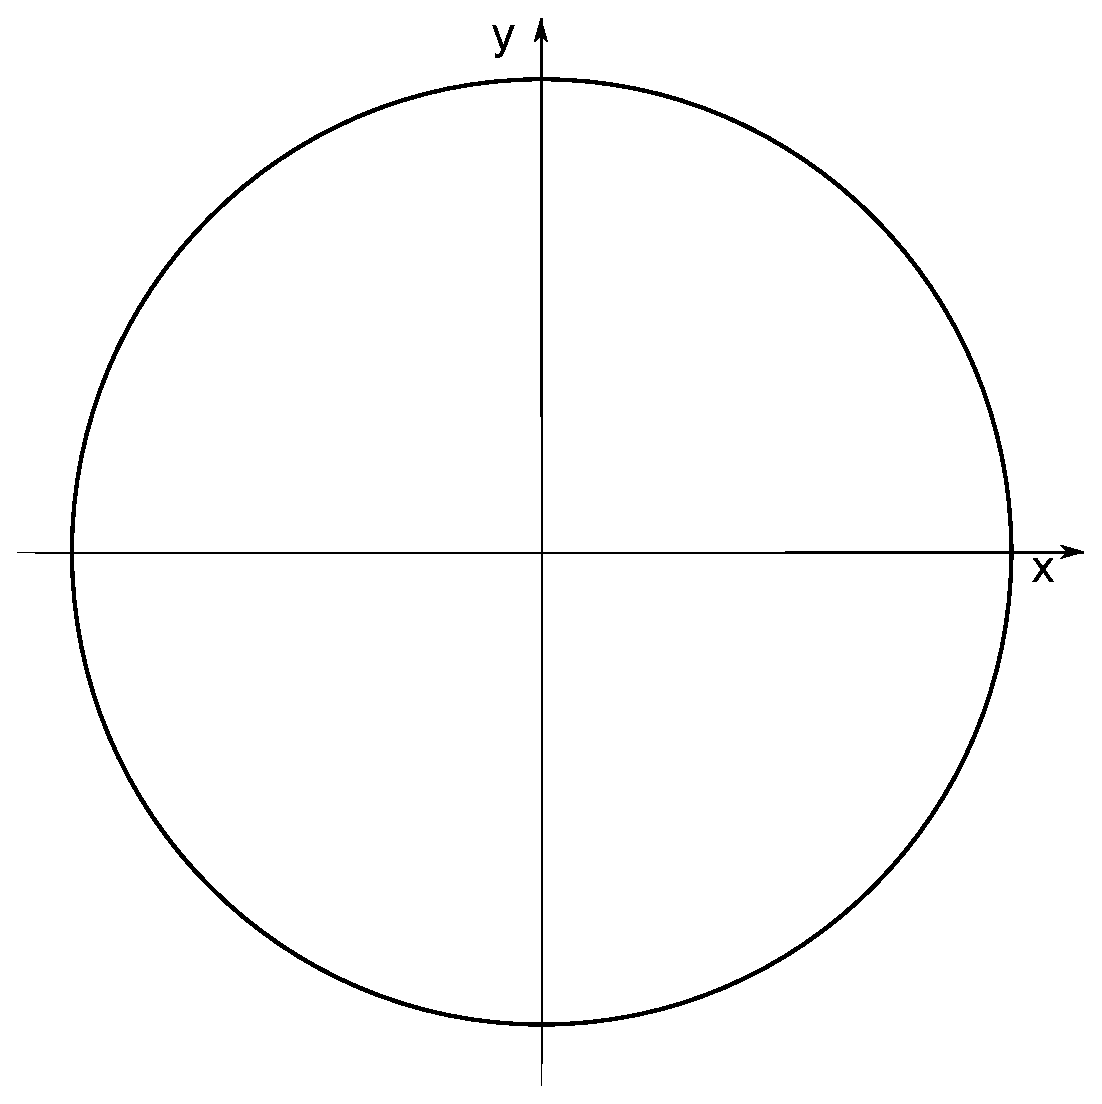
\includegraphics[width=6cm]{trig/img/blankCircle}

  Use the plot of the unit circle above, and sketch the angles that
  satisfy the equation above. Use the plot to determine the values of
  the angles in radians.

  \vfill

  \clearpage

\item Determine all values of $x$ that satisfy 
  \begin{eqnarray*}
    \tan(x^2+1) & = & \frac{\sqrt{3}}{3}.
  \end{eqnarray*}

  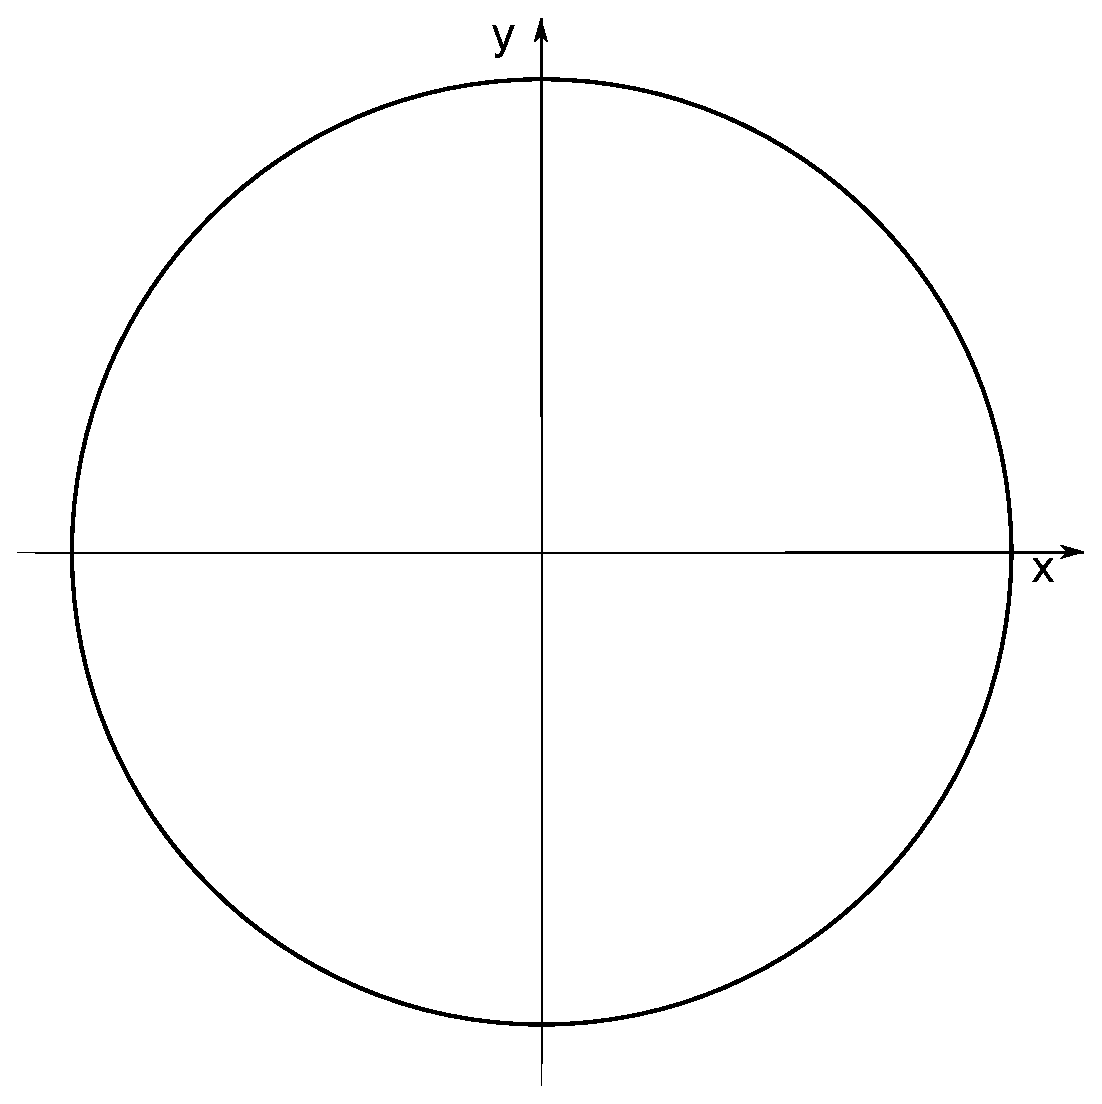
\includegraphics[width=6cm]{trig/img/blankCircle}

  Use the plot of the unit circle above, and sketch the angles that
  satisfy the equation above. Use the plot to determine the values of
  the angles in radians.

  \vfill

  \clearpage

\item The voltage within a circuit element is given by
  \begin{eqnarray*}
    V(t) & = & 100-50\cos\left( \frac{3\pi}{120} t + 3\pi \right).
  \end{eqnarray*}
  What is the minimum voltage and when does it occur? (Make a sketch
  of the unit circle!)

  \vfill
  
\end{problem}

\postClass

\begin{problem}
\item Briefly state two ideas from today's class.
  \begin{itemize}
  \item 
  \item 
  \end{itemize}
\item 
  \begin{subproblem}
    \item
  \end{subproblem}
\end{problem}


%%% Local Variables:
%%% mode: latex
%%% TeX-master: "../labManual"
%%% End:

